%!TEX root=../../sbc-template.tex

A detecção e o reconhecimento de objetos são componentes chave para a maioria dos sistemas de visão computacional e determinam o desempenho de muitos aplicativos, como rastreamento, recuperação, vigilância por vídeo e legendagem de imagens. O desempenho da detecção e reconhecimento de objetos depende muito da qualidade das características extraídas e da robustez dos modelos, uma vez que a aparência das imagens pode ser influenciada por diversos fatores, como condições de iluminação, pose, refletância dos objetos e características intrínsecas das câmeras \cite{Jiang:2019}. Por isso que, nos últimos anos, as redes neurais profundas ganharam espaço nos problemas mais complexos da atualidade como processamento de imagens e visão computacional. A Figura \ref{fig:example-detection} ilustra a detecção de várias classes para uma mesma entrada.

\begin{figure}[H]
    \centering
    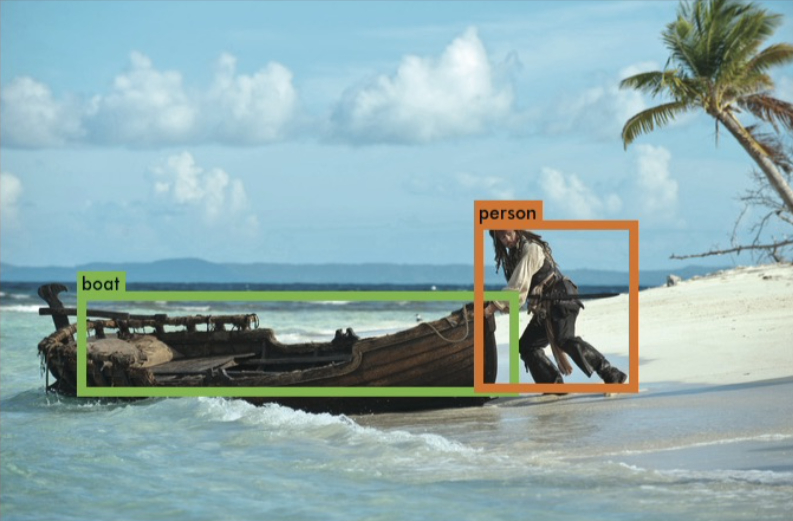
\includegraphics[width=.7\textwidth]{img/example-detection.png}
    \caption{Tarefa de detecção de objetos sendo realizada. Fonte: \cite{Yolo:2015}}
    \label{fig:example-detection}
\end{figure}

É importante salientar que a classificação de uma imagem, isto é, um modelo classificar o conteúdo de uma foto, por exemplo, é diferente de detectar exatamente em que área da foto o objeto encontra-se. Com isso, é possível perceber que os modelos que abordam essa tarefas precisam ser mais robustos pois existe agora uma nova etapa na qual o modelo precisa realizar: definir na imagem quais os limites da entidade em questão. Em resumo, o modelo, para detecção de objetos numa imagem, deve ser capaz de identificar a localização de uma ou mais entidades (as classes) além de emitir qual classe ela(s) pertence(m) \cite{Michelucci:2019}.

A métrica necessária para verificar a qualidade dessa tarefa é justamente a interseção da área correspondente ao objeto (resultado esperado) em relação à área detectada sobre a união dessas áreas em questão, conhecida também como Interseção sobre União (IoU) \cite{Chollet:2017}. O desafio está em detectar as áreas das entidades na imagem. Uma das primeiras estratégias que solucionaram esse problema é a Aproximação da Janela Deslizante: uma certa área (a janela deslizante) igual ou menor que a imagem total é inicialmente definida e percorre todas as combinações possíveis com a imagem original, calculando o IoU. Em seguida, outra janela deslizante é definida com outro tamanho e o processo é refeito. No fim, verifica-se qual IoU foi o mais satisfatório para o resultado final da detecção da entidade. Essa estratégia é bastante custosa pois podem existir milhares de combinações possíveis em cada teste, razão pela qual não é muito utilizada \cite{Michelucci:2019}.

Outra estratégia para a detecção é conhecida como Region-Based CNN (R-CNN), ou CNN Baseada em Regiões. Como a estratégia das janelas deslizantes necessita de muitas combinações, a baseada em regiões propõe inicialmente 2000 regiões na imagem. Em seguida as regiões adjacentes são unidas baseadas em características similares como cor, textura e forma, sendo possível visualizar a técnica na Figura \ref{fig:selective-search}. Então, com menos regiões para serem analisadas, o cálculo de IoU é também realizado e a melhor métrica acaba escolhendo também a melhor região para o resultado \cite{Michelucci:2019}.

\begin{figure}[H]
    \centering
    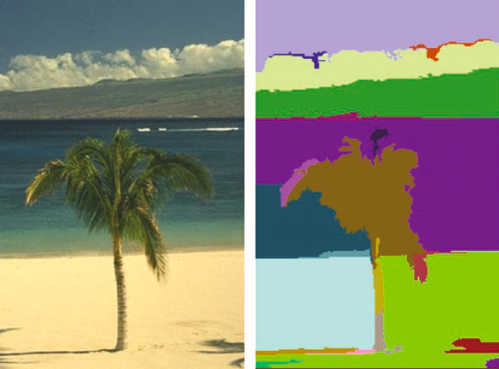
\includegraphics[width=.7\textwidth]{img/selective-search.png}
    \caption{Pesquisa seletiva destacando regiões de interesse. Fonte: \cite{Michelucci:2019}}
    \label{fig:selective-search}
\end{figure}

Como as R-CNN são modelos mais complexos devido ao janelamento, uma solução para torná-las mais rápidas foi desenvolvida: a chamada Fast R-CNN. A razão pela qual esse algoritmo é mais rápido que o R-CNN está no fato de que torna-se desnecessário alimentar 2000 propostas de região para a rede neural convolucional, o processo é realizado uma única vez com a extração de mapa de características da imagem, similar às características semelhantes das regiões inicializadas nas R-CNN \cite{Michelucci:2019}.

Mesmo as Fast R-CNN tendo se mostrado mais rápidas que as R-CNN convencionais, o custo para treinar o modelo ainda é alto visto que a pesquisa para selecionar as regiões propostas é ainda gargalo do algoritmo. Com isso, uma outra solução para essa etapa foi desenvolvida: utilizar uma outra rede neural para aprender as regiões de dados rotulados, removendo então a etapa demorada de procura seletiva das regiões. Assim, esse modelo foi chamado de Faster R-CNN por ser significativamente mais rápido que R-CNN e Fast R-CNN \cite{Michelucci:2019}.
